\documentclass{book}
\usepackage[a4paper,top=2.5cm,bottom=2.5cm,left=2.5cm,right=2.5cm]{geometry}
\usepackage{makeidx}
\usepackage{natbib}
\usepackage{graphicx}
\usepackage{multicol}
\usepackage{float}
\usepackage{listings}
\usepackage{color}
\usepackage{ifthen}
\usepackage[table]{xcolor}
\usepackage{textcomp}
\usepackage{alltt}
\usepackage{ifpdf}
\ifpdf
\usepackage[pdftex,
            pagebackref=true,
            colorlinks=true,
            linkcolor=blue,
            unicode
           ]{hyperref}
\else
\usepackage[ps2pdf,
            pagebackref=true,
            colorlinks=true,
            linkcolor=blue,
            unicode
           ]{hyperref}
\usepackage{pspicture}
\fi
\usepackage[utf8]{inputenc}
\usepackage[french]{babel}

\usepackage{mathptmx}
\usepackage[scaled=.90]{helvet}
\usepackage{courier}
\usepackage{sectsty}
\usepackage{amssymb}
\usepackage[titles]{tocloft}
\usepackage{doxygen}
\lstset{language=C++,inputencoding=utf8,basicstyle=\footnotesize,breaklines=true,breakatwhitespace=true,tabsize=4,numbers=left }
\makeindex
\setcounter{tocdepth}{3}
\renewcommand{\footrulewidth}{0.4pt}
\renewcommand{\familydefault}{\sfdefault}
\hfuzz=15pt
\setlength{\emergencystretch}{15pt}
\hbadness=750
\tolerance=750
\begin{document}
\hypersetup{pageanchor=false,citecolor=blue}
\begin{titlepage}
\vspace*{7cm}
\begin{center}
{\Large Drone\-Wifi \\[1ex]\large 0.\-5 }\\
\vspace*{1cm}
{\large Généré par Doxygen 1.8.3.1}\\
\vspace*{0.5cm}
{\small Mardi Février 19 2013 11:17:39}\\
\end{center}
\end{titlepage}
\clearemptydoublepage
\pagenumbering{roman}
\tableofcontents
\clearemptydoublepage
\pagenumbering{arabic}
\hypersetup{pageanchor=true,citecolor=blue}
\chapter{Index des espaces de nommage}
\section{Liste des espaces de nommage}
Liste de tous les espaces de nommage avec une brève description\-:\begin{DoxyCompactList}
\item\contentsline{section}{\hyperlink{namespace_ui}{Ui} }{\pageref{namespace_ui}}{}
\end{DoxyCompactList}

\chapter{Index hiérarchique}
\section{Hiérarchie des classes}
Cette liste d'héritage est classée approximativement par ordre alphabétique \-:\begin{DoxyCompactList}
\item \contentsline{section}{Q\-Main\-Window}{\pageref{class_q_main_window}}{}
\begin{DoxyCompactList}
\item \contentsline{section}{Main\-Window}{\pageref{class_main_window}}{}
\item \contentsline{section}{navdata\-Window}{\pageref{classnavdata_window}}{}
\end{DoxyCompactList}
\item \contentsline{section}{Q\-Thread}{\pageref{class_q_thread}}{}
\begin{DoxyCompactList}
\item \contentsline{section}{A\-R\-Drone}{\pageref{class_a_r_drone}}{}
\end{DoxyCompactList}
\end{DoxyCompactList}

\chapter{Index des classes}
\section{Structures de données}
Liste des structures de données avec une brève description \-:\begin{DoxyCompactList}
\item\contentsline{section}{\hyperlink{structardrone}{ardrone} }{\pageref{structardrone}}{}
\item\contentsline{section}{\hyperlink{class_a_r_drone}{A\-R\-Drone} }{\pageref{class_a_r_drone}}{}
\item\contentsline{section}{\hyperlink{structetat__commandes}{etat\-\_\-commandes} }{\pageref{structetat__commandes}}{}
\item\contentsline{section}{\hyperlink{class_main_window}{Main\-Window} }{\pageref{class_main_window}}{}
\item\contentsline{section}{\hyperlink{classnavdata_window}{navdata\-Window} }{\pageref{classnavdata_window}}{}
\item\contentsline{section}{\hyperlink{class_q_main_window}{Q\-Main\-Window} }{\pageref{class_q_main_window}}{}
\item\contentsline{section}{\hyperlink{class_q_thread}{Q\-Thread} }{\pageref{class_q_thread}}{}
\end{DoxyCompactList}

\chapter{Index des fichiers}
\section{Liste des fichiers}
Liste de tous les fichiers avec une brève description \-:\begin{DoxyCompactList}
\item\contentsline{section}{/media/\-D\-E\-V\-E\-L/\-Projet\-I\-U\-T/\-Drone\-Wifi/sources/keyboard\-Command/\hyperlink{ardrone_8cpp}{ardrone.\-cpp} }{\pageref{ardrone_8cpp}}{}
\item\contentsline{section}{/media/\-D\-E\-V\-E\-L/\-Projet\-I\-U\-T/\-Drone\-Wifi/sources/keyboard\-Command/\hyperlink{ardrone_8h}{ardrone.\-h} }{\pageref{ardrone_8h}}{}
\item\contentsline{section}{/media/\-D\-E\-V\-E\-L/\-Projet\-I\-U\-T/\-Drone\-Wifi/sources/keyboard\-Command/\hyperlink{main_8cpp}{main.\-cpp} }{\pageref{main_8cpp}}{}
\item\contentsline{section}{/media/\-D\-E\-V\-E\-L/\-Projet\-I\-U\-T/\-Drone\-Wifi/sources/keyboard\-Command/\hyperlink{mainwindow_8cpp}{mainwindow.\-cpp} }{\pageref{mainwindow_8cpp}}{}
\item\contentsline{section}{/media/\-D\-E\-V\-E\-L/\-Projet\-I\-U\-T/\-Drone\-Wifi/sources/keyboard\-Command/\hyperlink{mainwindow_8h}{mainwindow.\-h} }{\pageref{mainwindow_8h}}{}
\item\contentsline{section}{/media/\-D\-E\-V\-E\-L/\-Projet\-I\-U\-T/\-Drone\-Wifi/sources/keyboard\-Command/\hyperlink{navdatawindow_8cpp}{navdatawindow.\-cpp} }{\pageref{navdatawindow_8cpp}}{}
\item\contentsline{section}{/media/\-D\-E\-V\-E\-L/\-Projet\-I\-U\-T/\-Drone\-Wifi/sources/keyboard\-Command/\hyperlink{navdatawindow_8h}{navdatawindow.\-h} }{\pageref{navdatawindow_8h}}{}
\item\contentsline{section}{/media/\-D\-E\-V\-E\-L/\-Projet\-I\-U\-T/\-Drone\-Wifi/sources/wifi/\hyperlink{connexion_8c}{connexion.\-c} }{\pageref{connexion_8c}}{}
\end{DoxyCompactList}

\chapter{Documentation des espaces de nommage}
\hypertarget{namespace_ui}{\section{Référence de l'espace de nommage Ui}
\label{namespace_ui}\index{Ui@{Ui}}
}

\chapter{Documentation des classes}
\hypertarget{class_a_r_drone}{\section{Référence de la classe A\-R\-Drone}
\label{class_a_r_drone}\index{A\-R\-Drone@{A\-R\-Drone}}
}


{\ttfamily \#include $<$ardrone.\-h$>$}



Graphe d'héritage de A\-R\-Drone\-:
\nopagebreak
\begin{figure}[H]
\begin{center}
\leavevmode
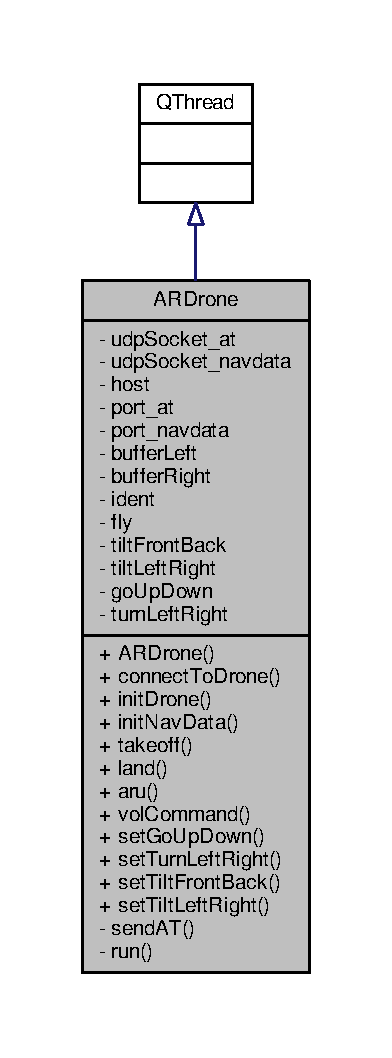
\includegraphics[width=184pt]{class_a_r_drone__inherit__graph}
\end{center}
\end{figure}


Graphe de collaboration de A\-R\-Drone\-:
\nopagebreak
\begin{figure}[H]
\begin{center}
\leavevmode
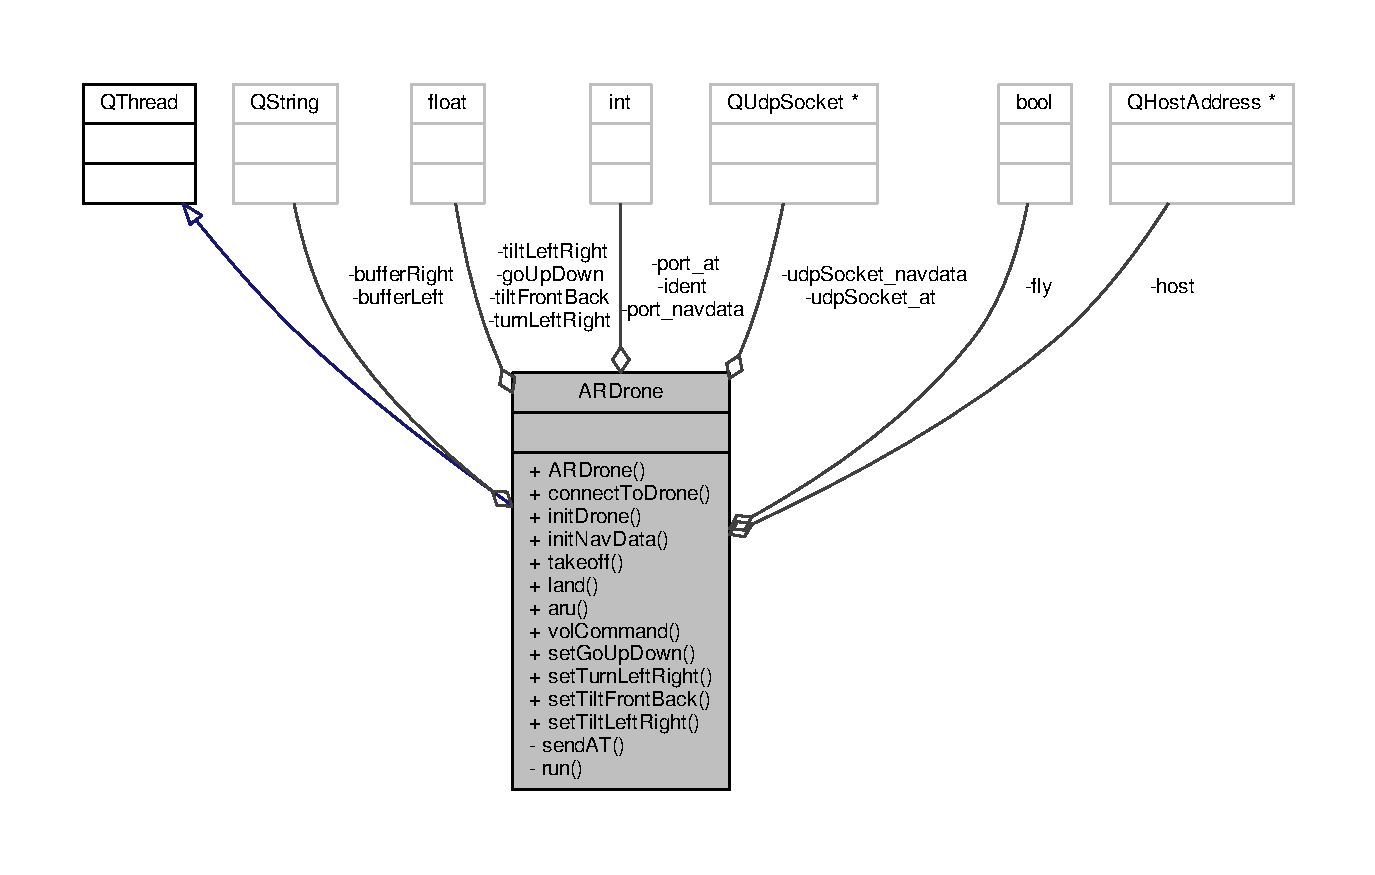
\includegraphics[width=184pt]{class_a_r_drone__coll__graph}
\end{center}
\end{figure}
\subsection*{Fonctions membres publiques}
\begin{DoxyCompactItemize}
\item 
\hyperlink{class_a_r_drone_a9f5df81d1e4b136238e7b89b03cf915b}{A\-R\-Drone} (Q\-Object $\ast$parent=0)
\item 
bool \hyperlink{class_a_r_drone_a0ba4b4e4cf7a107a1587152af3f4fbab}{connect\-To\-Drone} (void)
\begin{DoxyCompactList}\small\item\em Initialise la connexion au drone. \end{DoxyCompactList}\item 
bool \hyperlink{class_a_r_drone_ab447af60c30509710f55922ff07fc3a4}{init\-Drone} (void)
\begin{DoxyCompactList}\small\item\em Initialise le drone (à utiliser avant de lancer la navigation) \end{DoxyCompactList}\item 
bool \hyperlink{class_a_r_drone_a36946b429549afb5b1d64c0ff1fe4fbb}{init\-Nav\-Data} (void)
\begin{DoxyCompactList}\small\item\em Initialise le fux de données. \end{DoxyCompactList}\item 
bool \hyperlink{class_a_r_drone_a34d3e2ff71b9fc05e2faa20015d320c8}{takeoff} (void)
\begin{DoxyCompactList}\small\item\em Demande de décollage. \end{DoxyCompactList}\item 
bool \hyperlink{class_a_r_drone_a4735e9dbf7f8c0c43a6e4f55511d7262}{land} (void)
\begin{DoxyCompactList}\small\item\em Demande d'atterrissage. \end{DoxyCompactList}\item 
bool \hyperlink{class_a_r_drone_ac0bf02a934602af7eb48e20e2717bb3e}{aru} (void)
\begin{DoxyCompactList}\small\item\em Demande d'arrêt d'urgence. \end{DoxyCompactList}\item 
bool \hyperlink{class_a_r_drone_a4a3c6bdd5043578998f074ca7a85d146}{vol\-Command} (float tilt\-Left\-Right\-\_\-, float tilt\-Front\-Back\-\_\-, float go\-Up\-Down\-\_\-, float turn\-Left\-Right\-\_\-)
\begin{DoxyCompactList}\small\item\em Pilotage du drone en vol. \end{DoxyCompactList}\item 
void \hyperlink{class_a_r_drone_a40d5afd3a519061379938368c9096df0}{set\-Go\-Up\-Down} (float val)
\begin{DoxyCompactList}\small\item\em Setter sécurisé de la valeur de la vitesse verticale. \end{DoxyCompactList}\item 
void \hyperlink{class_a_r_drone_a846d9ca708547b77d6353b8c544e2764}{set\-Turn\-Left\-Right} (float val)
\begin{DoxyCompactList}\small\item\em Setter sécurisé de la valeur de la vitesse angulaire. \end{DoxyCompactList}\item 
void \hyperlink{class_a_r_drone_a35091a8252bbb1cffab5c07834d1f263}{set\-Tilt\-Front\-Back} (float val)
\begin{DoxyCompactList}\small\item\em Setter sécurisé de la valeur de l'inclinaison avant arrière. \end{DoxyCompactList}\item 
void \hyperlink{class_a_r_drone_a2cd513a18603d81fdbc8167c103af577}{set\-Tilt\-Left\-Right} (float val)
\begin{DoxyCompactList}\small\item\em Setter sécurisé de la valeur de l'inclinaison gauche droite. \end{DoxyCompactList}\end{DoxyCompactItemize}


\subsection{Description détaillée}


Définition à la ligne 9 du fichier ardrone.\-h.



\subsection{Documentation des constructeurs et destructeur}
\hypertarget{class_a_r_drone_a9f5df81d1e4b136238e7b89b03cf915b}{\index{A\-R\-Drone@{A\-R\-Drone}!A\-R\-Drone@{A\-R\-Drone}}
\index{A\-R\-Drone@{A\-R\-Drone}!ARDrone@{A\-R\-Drone}}
\subsubsection[{A\-R\-Drone}]{\setlength{\rightskip}{0pt plus 5cm}{\bf A\-R\-Drone} (
\begin{DoxyParamCaption}
\item[{Q\-Object $\ast$}]{parent = {\ttfamily 0}}
\end{DoxyParamCaption}
)\hspace{0.3cm}{\ttfamily [explicit]}}}\label{class_a_r_drone_a9f5df81d1e4b136238e7b89b03cf915b}


Définition à la ligne 3 du fichier ardrone.\-cpp.



\subsection{Documentation des fonctions membres}
\hypertarget{class_a_r_drone_ac0bf02a934602af7eb48e20e2717bb3e}{\index{A\-R\-Drone@{A\-R\-Drone}!aru@{aru}}
\index{aru@{aru}!ARDrone@{A\-R\-Drone}}
\subsubsection[{aru}]{\setlength{\rightskip}{0pt plus 5cm}bool aru (
\begin{DoxyParamCaption}
\item[{void}]{}
\end{DoxyParamCaption}
)}}\label{class_a_r_drone_ac0bf02a934602af7eb48e20e2717bb3e}


Demande d'arrêt d'urgence. 

\begin{DoxyReturn}{Renvoie}
(bool) true \-: demande envoyée ; false \-: demande non-\/envoyée 
\end{DoxyReturn}


Définition à la ligne 111 du fichier ardrone.\-cpp.

\hypertarget{class_a_r_drone_a0ba4b4e4cf7a107a1587152af3f4fbab}{\index{A\-R\-Drone@{A\-R\-Drone}!connect\-To\-Drone@{connect\-To\-Drone}}
\index{connect\-To\-Drone@{connect\-To\-Drone}!ARDrone@{A\-R\-Drone}}
\subsubsection[{connect\-To\-Drone}]{\setlength{\rightskip}{0pt plus 5cm}bool connect\-To\-Drone (
\begin{DoxyParamCaption}
\item[{void}]{}
\end{DoxyParamCaption}
)}}\label{class_a_r_drone_a0ba4b4e4cf7a107a1587152af3f4fbab}


Initialise la connexion au drone. 

\begin{DoxyReturn}{Renvoie}
(bool) true \-: Connexion réussie ; false \-: Connexion échouée 
\end{DoxyReturn}
\begin{DoxyAuthor}{Auteur}
Baudouin Feildel 
\end{DoxyAuthor}


Définition à la ligne 15 du fichier ardrone.\-cpp.



Voici le graphe des appelants de cette fonction \-:
\nopagebreak
\begin{figure}[H]
\begin{center}
\leavevmode
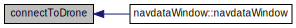
\includegraphics[width=350pt]{class_a_r_drone_a0ba4b4e4cf7a107a1587152af3f4fbab_icgraph}
\end{center}
\end{figure}


\hypertarget{class_a_r_drone_ab447af60c30509710f55922ff07fc3a4}{\index{A\-R\-Drone@{A\-R\-Drone}!init\-Drone@{init\-Drone}}
\index{init\-Drone@{init\-Drone}!ARDrone@{A\-R\-Drone}}
\subsubsection[{init\-Drone}]{\setlength{\rightskip}{0pt plus 5cm}bool init\-Drone (
\begin{DoxyParamCaption}
\item[{void}]{}
\end{DoxyParamCaption}
)}}\label{class_a_r_drone_ab447af60c30509710f55922ff07fc3a4}


Initialise le drone (à utiliser avant de lancer la navigation) 

\begin{DoxyReturn}{Renvoie}
(bool) true \-: Initialisation réussie ; false \-: Initialisation échouée 
\end{DoxyReturn}
\begin{DoxyAuthor}{Auteur}
Baudouin Feildel 
\end{DoxyAuthor}


Définition à la ligne 35 du fichier ardrone.\-cpp.

\hypertarget{class_a_r_drone_a36946b429549afb5b1d64c0ff1fe4fbb}{\index{A\-R\-Drone@{A\-R\-Drone}!init\-Nav\-Data@{init\-Nav\-Data}}
\index{init\-Nav\-Data@{init\-Nav\-Data}!ARDrone@{A\-R\-Drone}}
\subsubsection[{init\-Nav\-Data}]{\setlength{\rightskip}{0pt plus 5cm}bool init\-Nav\-Data (
\begin{DoxyParamCaption}
\item[{void}]{}
\end{DoxyParamCaption}
)}}\label{class_a_r_drone_a36946b429549afb5b1d64c0ff1fe4fbb}


Initialise le fux de données. 

\begin{DoxyReturn}{Renvoie}
(bool) true \-: Initialisation réussie ; false \-: Initialisation échouée 
\end{DoxyReturn}
\begin{DoxyAuthor}{Auteur}
Baudouin Feildel 
\end{DoxyAuthor}


Définition à la ligne 51 du fichier ardrone.\-cpp.



Voici le graphe des appelants de cette fonction \-:
\nopagebreak
\begin{figure}[H]
\begin{center}
\leavevmode
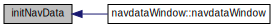
\includegraphics[width=346pt]{class_a_r_drone_a36946b429549afb5b1d64c0ff1fe4fbb_icgraph}
\end{center}
\end{figure}


\hypertarget{class_a_r_drone_a4735e9dbf7f8c0c43a6e4f55511d7262}{\index{A\-R\-Drone@{A\-R\-Drone}!land@{land}}
\index{land@{land}!ARDrone@{A\-R\-Drone}}
\subsubsection[{land}]{\setlength{\rightskip}{0pt plus 5cm}bool land (
\begin{DoxyParamCaption}
\item[{void}]{}
\end{DoxyParamCaption}
)}}\label{class_a_r_drone_a4735e9dbf7f8c0c43a6e4f55511d7262}


Demande d'atterrissage. 

\begin{DoxyReturn}{Renvoie}
(bool) true \-: demande envoyée ; false \-: demande non-\/envoyée 
\end{DoxyReturn}


Définition à la ligne 101 du fichier ardrone.\-cpp.

\hypertarget{class_a_r_drone_a40d5afd3a519061379938368c9096df0}{\index{A\-R\-Drone@{A\-R\-Drone}!set\-Go\-Up\-Down@{set\-Go\-Up\-Down}}
\index{set\-Go\-Up\-Down@{set\-Go\-Up\-Down}!ARDrone@{A\-R\-Drone}}
\subsubsection[{set\-Go\-Up\-Down}]{\setlength{\rightskip}{0pt plus 5cm}void set\-Go\-Up\-Down (
\begin{DoxyParamCaption}
\item[{float}]{val}
\end{DoxyParamCaption}
)\hspace{0.3cm}{\ttfamily [inline]}}}\label{class_a_r_drone_a40d5afd3a519061379938368c9096df0}


Setter sécurisé de la valeur de la vitesse verticale. 


\begin{DoxyParams}{Paramètres}
{\em float} & val \-: valeur à écrire \\
\hline
\end{DoxyParams}
\begin{DoxyAuthor}{Auteur}
Baudouin Feildel 
\end{DoxyAuthor}


Définition à la ligne 79 du fichier ardrone.\-h.



Voici le graphe des appelants de cette fonction \-:
\nopagebreak
\begin{figure}[H]
\begin{center}
\leavevmode
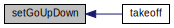
\includegraphics[width=246pt]{class_a_r_drone_a40d5afd3a519061379938368c9096df0_icgraph}
\end{center}
\end{figure}


\hypertarget{class_a_r_drone_a35091a8252bbb1cffab5c07834d1f263}{\index{A\-R\-Drone@{A\-R\-Drone}!set\-Tilt\-Front\-Back@{set\-Tilt\-Front\-Back}}
\index{set\-Tilt\-Front\-Back@{set\-Tilt\-Front\-Back}!ARDrone@{A\-R\-Drone}}
\subsubsection[{set\-Tilt\-Front\-Back}]{\setlength{\rightskip}{0pt plus 5cm}void set\-Tilt\-Front\-Back (
\begin{DoxyParamCaption}
\item[{float}]{val}
\end{DoxyParamCaption}
)\hspace{0.3cm}{\ttfamily [inline]}}}\label{class_a_r_drone_a35091a8252bbb1cffab5c07834d1f263}


Setter sécurisé de la valeur de l'inclinaison avant arrière. 


\begin{DoxyParams}{Paramètres}
{\em float} & val \-: valeur à écrire \\
\hline
\end{DoxyParams}
\begin{DoxyAuthor}{Auteur}
Baudouin Feildel 
\end{DoxyAuthor}


Définition à la ligne 95 du fichier ardrone.\-h.



Voici le graphe des appelants de cette fonction \-:
\nopagebreak
\begin{figure}[H]
\begin{center}
\leavevmode
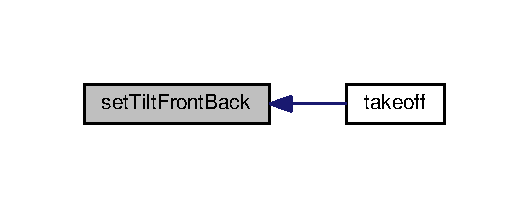
\includegraphics[width=254pt]{class_a_r_drone_a35091a8252bbb1cffab5c07834d1f263_icgraph}
\end{center}
\end{figure}


\hypertarget{class_a_r_drone_a2cd513a18603d81fdbc8167c103af577}{\index{A\-R\-Drone@{A\-R\-Drone}!set\-Tilt\-Left\-Right@{set\-Tilt\-Left\-Right}}
\index{set\-Tilt\-Left\-Right@{set\-Tilt\-Left\-Right}!ARDrone@{A\-R\-Drone}}
\subsubsection[{set\-Tilt\-Left\-Right}]{\setlength{\rightskip}{0pt plus 5cm}void set\-Tilt\-Left\-Right (
\begin{DoxyParamCaption}
\item[{float}]{val}
\end{DoxyParamCaption}
)\hspace{0.3cm}{\ttfamily [inline]}}}\label{class_a_r_drone_a2cd513a18603d81fdbc8167c103af577}


Setter sécurisé de la valeur de l'inclinaison gauche droite. 


\begin{DoxyParams}{Paramètres}
{\em float} & val \-: valeur à écrire \\
\hline
\end{DoxyParams}
\begin{DoxyAuthor}{Auteur}
Baudouin Feildel 
\end{DoxyAuthor}


Définition à la ligne 103 du fichier ardrone.\-h.



Voici le graphe des appelants de cette fonction \-:
\nopagebreak
\begin{figure}[H]
\begin{center}
\leavevmode
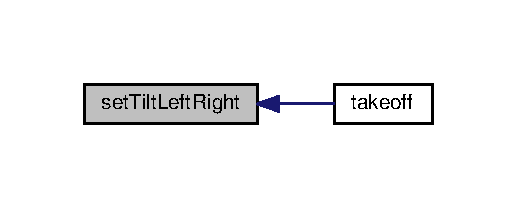
\includegraphics[width=248pt]{class_a_r_drone_a2cd513a18603d81fdbc8167c103af577_icgraph}
\end{center}
\end{figure}


\hypertarget{class_a_r_drone_a846d9ca708547b77d6353b8c544e2764}{\index{A\-R\-Drone@{A\-R\-Drone}!set\-Turn\-Left\-Right@{set\-Turn\-Left\-Right}}
\index{set\-Turn\-Left\-Right@{set\-Turn\-Left\-Right}!ARDrone@{A\-R\-Drone}}
\subsubsection[{set\-Turn\-Left\-Right}]{\setlength{\rightskip}{0pt plus 5cm}void set\-Turn\-Left\-Right (
\begin{DoxyParamCaption}
\item[{float}]{val}
\end{DoxyParamCaption}
)\hspace{0.3cm}{\ttfamily [inline]}}}\label{class_a_r_drone_a846d9ca708547b77d6353b8c544e2764}


Setter sécurisé de la valeur de la vitesse angulaire. 


\begin{DoxyParams}{Paramètres}
{\em float} & val \-: valeur à écrire \\
\hline
\end{DoxyParams}
\begin{DoxyAuthor}{Auteur}
Baudouin Feildel 
\end{DoxyAuthor}


Définition à la ligne 87 du fichier ardrone.\-h.



Voici le graphe des appelants de cette fonction \-:
\nopagebreak
\begin{figure}[H]
\begin{center}
\leavevmode
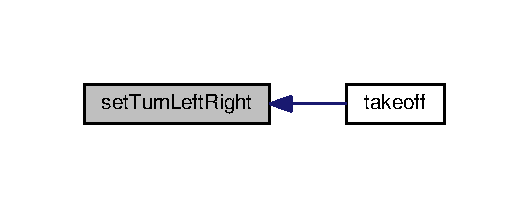
\includegraphics[width=254pt]{class_a_r_drone_a846d9ca708547b77d6353b8c544e2764_icgraph}
\end{center}
\end{figure}


\hypertarget{class_a_r_drone_a34d3e2ff71b9fc05e2faa20015d320c8}{\index{A\-R\-Drone@{A\-R\-Drone}!takeoff@{takeoff}}
\index{takeoff@{takeoff}!ARDrone@{A\-R\-Drone}}
\subsubsection[{takeoff}]{\setlength{\rightskip}{0pt plus 5cm}bool takeoff (
\begin{DoxyParamCaption}
\item[{void}]{}
\end{DoxyParamCaption}
)}}\label{class_a_r_drone_a34d3e2ff71b9fc05e2faa20015d320c8}


Demande de décollage. 

\begin{DoxyReturn}{Renvoie}
(bool) true \-: demande envoyée ; false \-: demande non-\/envoyée 
\end{DoxyReturn}
\begin{DoxyAuthor}{Auteur}
Baudouin Feildel 
\end{DoxyAuthor}


Définition à la ligne 80 du fichier ardrone.\-cpp.



Voici le graphe d'appel pour cette fonction \-:
\nopagebreak
\begin{figure}[H]
\begin{center}
\leavevmode
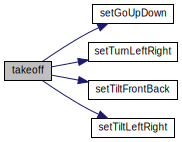
\includegraphics[width=254pt]{class_a_r_drone_a34d3e2ff71b9fc05e2faa20015d320c8_cgraph}
\end{center}
\end{figure}


\hypertarget{class_a_r_drone_a4a3c6bdd5043578998f074ca7a85d146}{\index{A\-R\-Drone@{A\-R\-Drone}!vol\-Command@{vol\-Command}}
\index{vol\-Command@{vol\-Command}!ARDrone@{A\-R\-Drone}}
\subsubsection[{vol\-Command}]{\setlength{\rightskip}{0pt plus 5cm}bool vol\-Command (
\begin{DoxyParamCaption}
\item[{float}]{tilt\-Left\-Right\-\_\-, }
\item[{float}]{tilt\-Front\-Back\-\_\-, }
\item[{float}]{go\-Up\-Down\-\_\-, }
\item[{float}]{turn\-Left\-Right\-\_\-}
\end{DoxyParamCaption}
)}}\label{class_a_r_drone_a4a3c6bdd5043578998f074ca7a85d146}


Pilotage du drone en vol. 


\begin{DoxyParams}{Paramètres}
{\em float} & tilt\-Left\-Right\-\_\- Inclinaison gauche droite ; \mbox{[}-\/1,1\mbox{]} \\
\hline
{\em float} & tilt\-Front\-Back\-\_\- Inclinaison avant arrière ; \mbox{[}-\/1;1\mbox{]} \\
\hline
{\em float} & go\-Up\-Down\-\_\- Vitesse verticale ; \mbox{[}-\/1;1\mbox{]} \\
\hline
{\em float} & turn\-Left\-Right\-\_\- Vitesse angulaire ; \mbox{[}-\/1;1\mbox{]} \\
\hline
\end{DoxyParams}
\begin{DoxyReturn}{Renvoie}
(bool) true \-: commande envoyée ; false \-: commande non-\/envoyée 
\end{DoxyReturn}
\begin{DoxyAuthor}{Auteur}
Baudouin Feildel 
\end{DoxyAuthor}


Définition à la ligne 121 du fichier ardrone.\-cpp.



La documentation de cette classe a été générée à partir des fichiers suivants \-:\begin{DoxyCompactItemize}
\item 
/media/\-D\-E\-V\-E\-L/\-Projet\-I\-U\-T/\-Drone\-Wifi/sources/keyboard\-Command/\hyperlink{ardrone_8h}{ardrone.\-h}\item 
/media/\-D\-E\-V\-E\-L/\-Projet\-I\-U\-T/\-Drone\-Wifi/sources/keyboard\-Command/\hyperlink{ardrone_8cpp}{ardrone.\-cpp}\end{DoxyCompactItemize}

\hypertarget{class_main_window}{\section{Référence de la classe Main\-Window}
\label{class_main_window}\index{Main\-Window@{Main\-Window}}
}


{\ttfamily \#include $<$mainwindow.\-h$>$}



Graphe d'héritage de Main\-Window\-:
\nopagebreak
\begin{figure}[H]
\begin{center}
\leavevmode
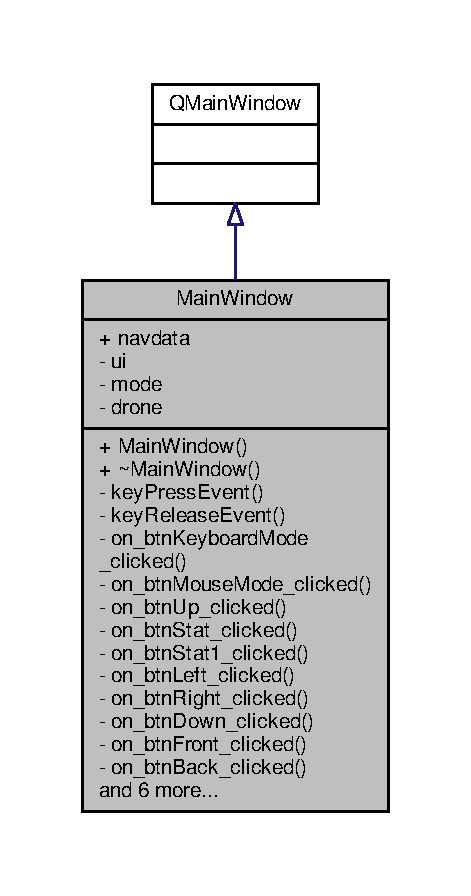
\includegraphics[width=174pt]{class_main_window__inherit__graph}
\end{center}
\end{figure}


Graphe de collaboration de Main\-Window\-:
\nopagebreak
\begin{figure}[H]
\begin{center}
\leavevmode
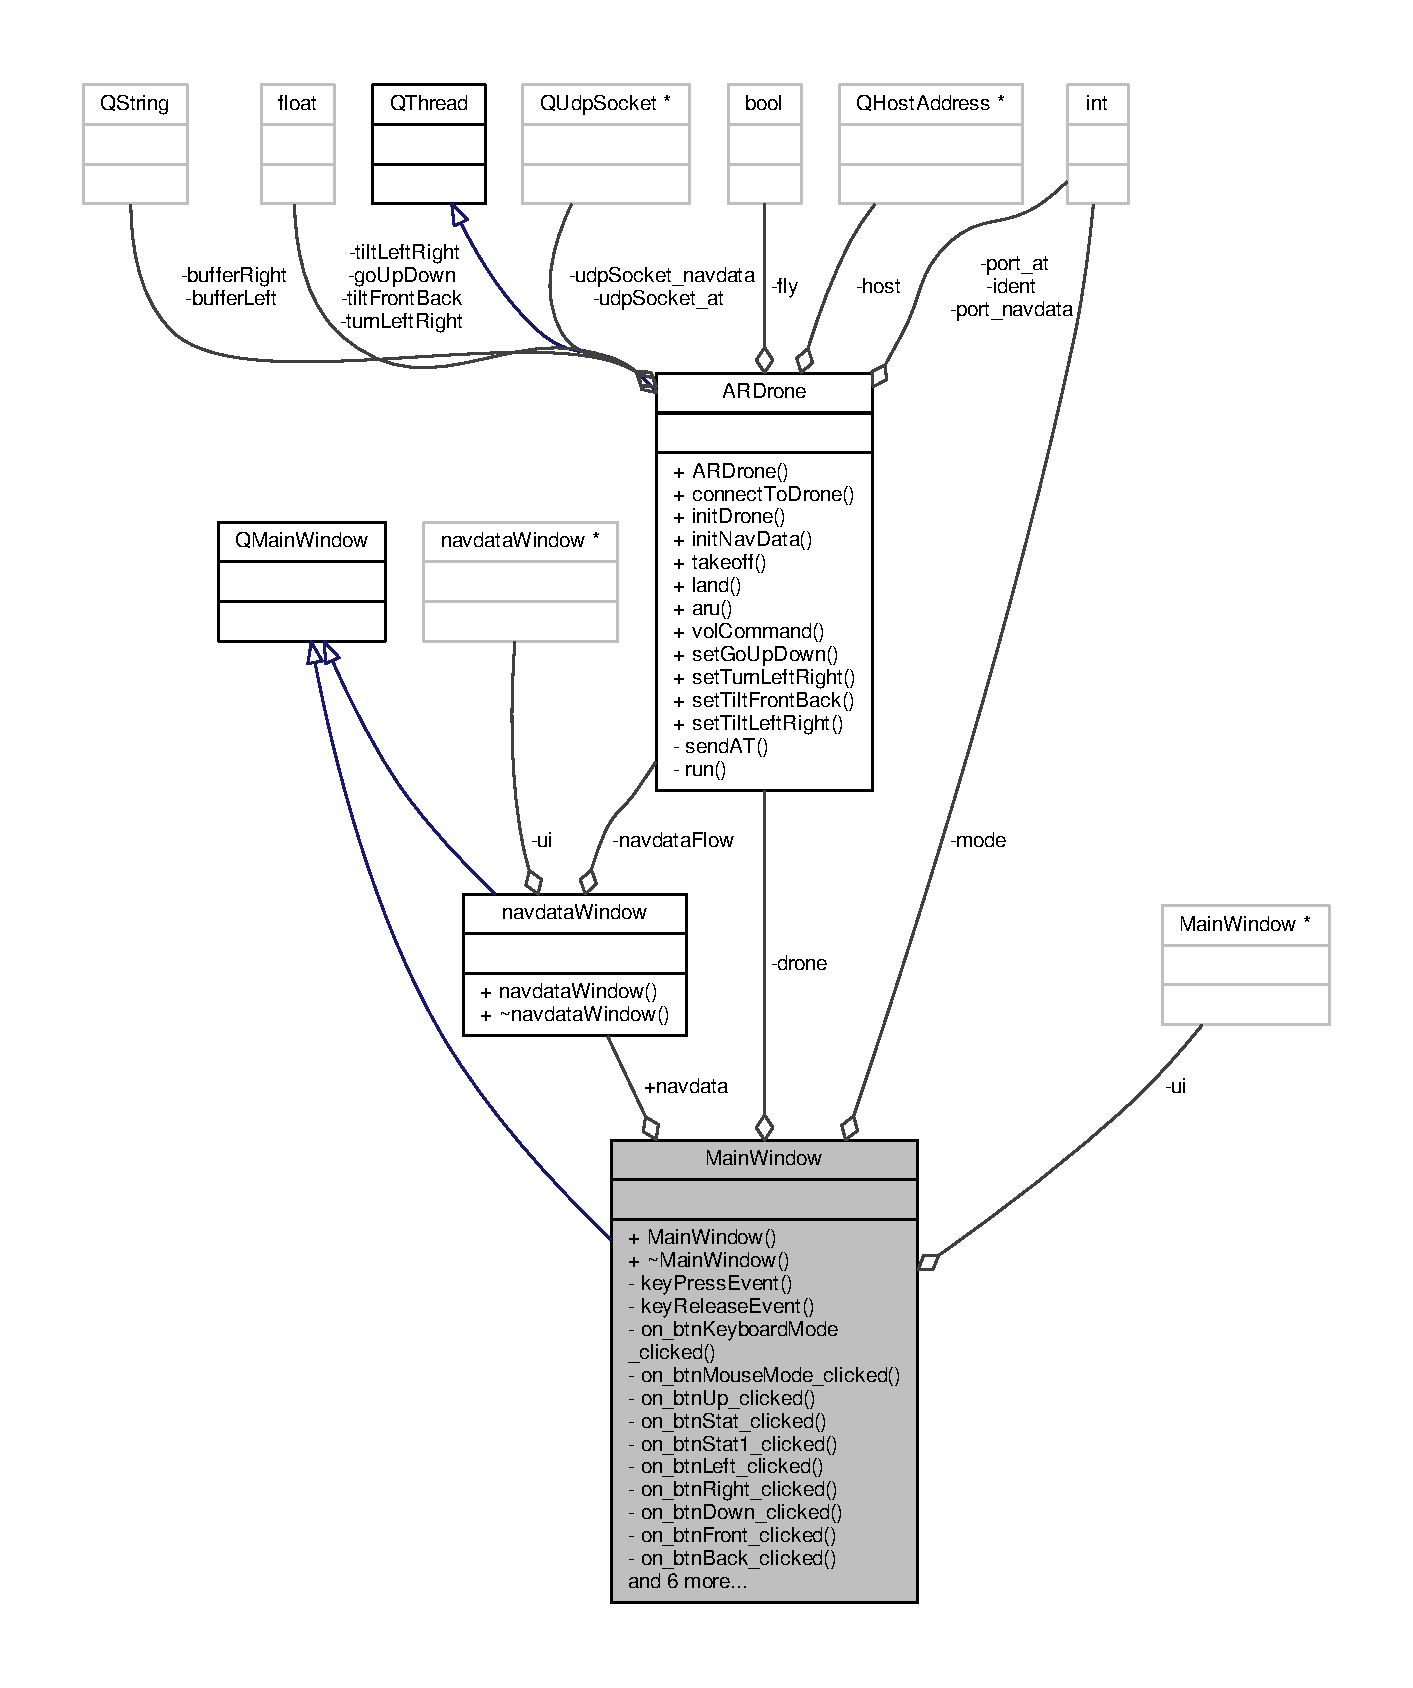
\includegraphics[width=246pt]{class_main_window__coll__graph}
\end{center}
\end{figure}
\subsection*{Fonctions membres publiques}
\begin{DoxyCompactItemize}
\item 
\hyperlink{class_main_window_a46f32c7a0b51359e13505396ce9b316b}{Main\-Window} (Q\-Widget $\ast$parent=0)
\item 
\hyperlink{class_main_window_aa33fa7d45aa34b9ede5cb69ab574a1b2}{$\sim$\-Main\-Window} ()
\end{DoxyCompactItemize}
\subsection*{Champs de données}
\begin{DoxyCompactItemize}
\item 
\hyperlink{classnavdata_window}{navdata\-Window} $\ast$ \hyperlink{class_main_window_a2e8ccc2fc320190b3aed244f54822982}{navdata}
\end{DoxyCompactItemize}


\subsection{Description détaillée}


Définition à la ligne 13 du fichier mainwindow.\-h.



\subsection{Documentation des constructeurs et destructeur}
\hypertarget{class_main_window_a46f32c7a0b51359e13505396ce9b316b}{\index{Main\-Window@{Main\-Window}!Main\-Window@{Main\-Window}}
\index{Main\-Window@{Main\-Window}!MainWindow@{Main\-Window}}
\subsubsection[{Main\-Window}]{\setlength{\rightskip}{0pt plus 5cm}{\bf Main\-Window} (
\begin{DoxyParamCaption}
\item[{Q\-Widget $\ast$}]{parent = {\ttfamily 0}}
\end{DoxyParamCaption}
)\hspace{0.3cm}{\ttfamily [explicit]}}}\label{class_main_window_a46f32c7a0b51359e13505396ce9b316b}


Définition à la ligne 4 du fichier mainwindow.\-cpp.

\hypertarget{class_main_window_aa33fa7d45aa34b9ede5cb69ab574a1b2}{\index{Main\-Window@{Main\-Window}!$\sim$\-Main\-Window@{$\sim$\-Main\-Window}}
\index{$\sim$\-Main\-Window@{$\sim$\-Main\-Window}!MainWindow@{Main\-Window}}
\subsubsection[{$\sim$\-Main\-Window}]{\setlength{\rightskip}{0pt plus 5cm}$\sim${\bf Main\-Window} (
\begin{DoxyParamCaption}
{}
\end{DoxyParamCaption}
)}}\label{class_main_window_aa33fa7d45aa34b9ede5cb69ab574a1b2}


Définition à la ligne 13 du fichier mainwindow.\-cpp.



\subsection{Documentation des champs}
\hypertarget{class_main_window_a2e8ccc2fc320190b3aed244f54822982}{\index{Main\-Window@{Main\-Window}!navdata@{navdata}}
\index{navdata@{navdata}!MainWindow@{Main\-Window}}
\subsubsection[{navdata}]{\setlength{\rightskip}{0pt plus 5cm}{\bf navdata\-Window}$\ast$ navdata}}\label{class_main_window_a2e8ccc2fc320190b3aed244f54822982}


Définition à la ligne 19 du fichier mainwindow.\-h.



La documentation de cette classe a été générée à partir des fichiers suivants \-:\begin{DoxyCompactItemize}
\item 
/media/\-D\-E\-V\-E\-L/\-Projet\-I\-U\-T/\-Drone\-Wifi/sources/keyboard\-Command/\hyperlink{mainwindow_8h}{mainwindow.\-h}\item 
/media/\-D\-E\-V\-E\-L/\-Projet\-I\-U\-T/\-Drone\-Wifi/sources/keyboard\-Command/\hyperlink{mainwindow_8cpp}{mainwindow.\-cpp}\end{DoxyCompactItemize}

\hypertarget{classnavdata_window}{\section{Référence de la classe navdata\-Window}
\label{classnavdata_window}\index{navdata\-Window@{navdata\-Window}}
}


{\ttfamily \#include $<$navdatawindow.\-h$>$}



Graphe d'héritage de navdata\-Window\-:
\nopagebreak
\begin{figure}[H]
\begin{center}
\leavevmode
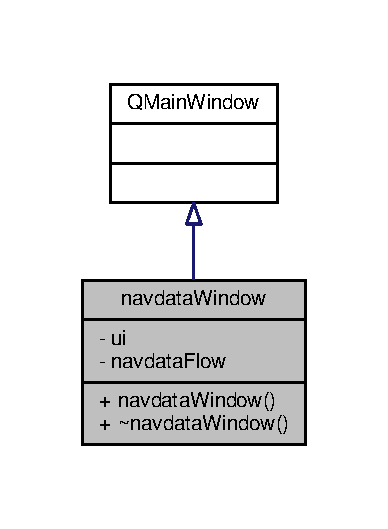
\includegraphics[width=186pt]{classnavdata_window__inherit__graph}
\end{center}
\end{figure}


Graphe de collaboration de navdata\-Window\-:
\nopagebreak
\begin{figure}[H]
\begin{center}
\leavevmode
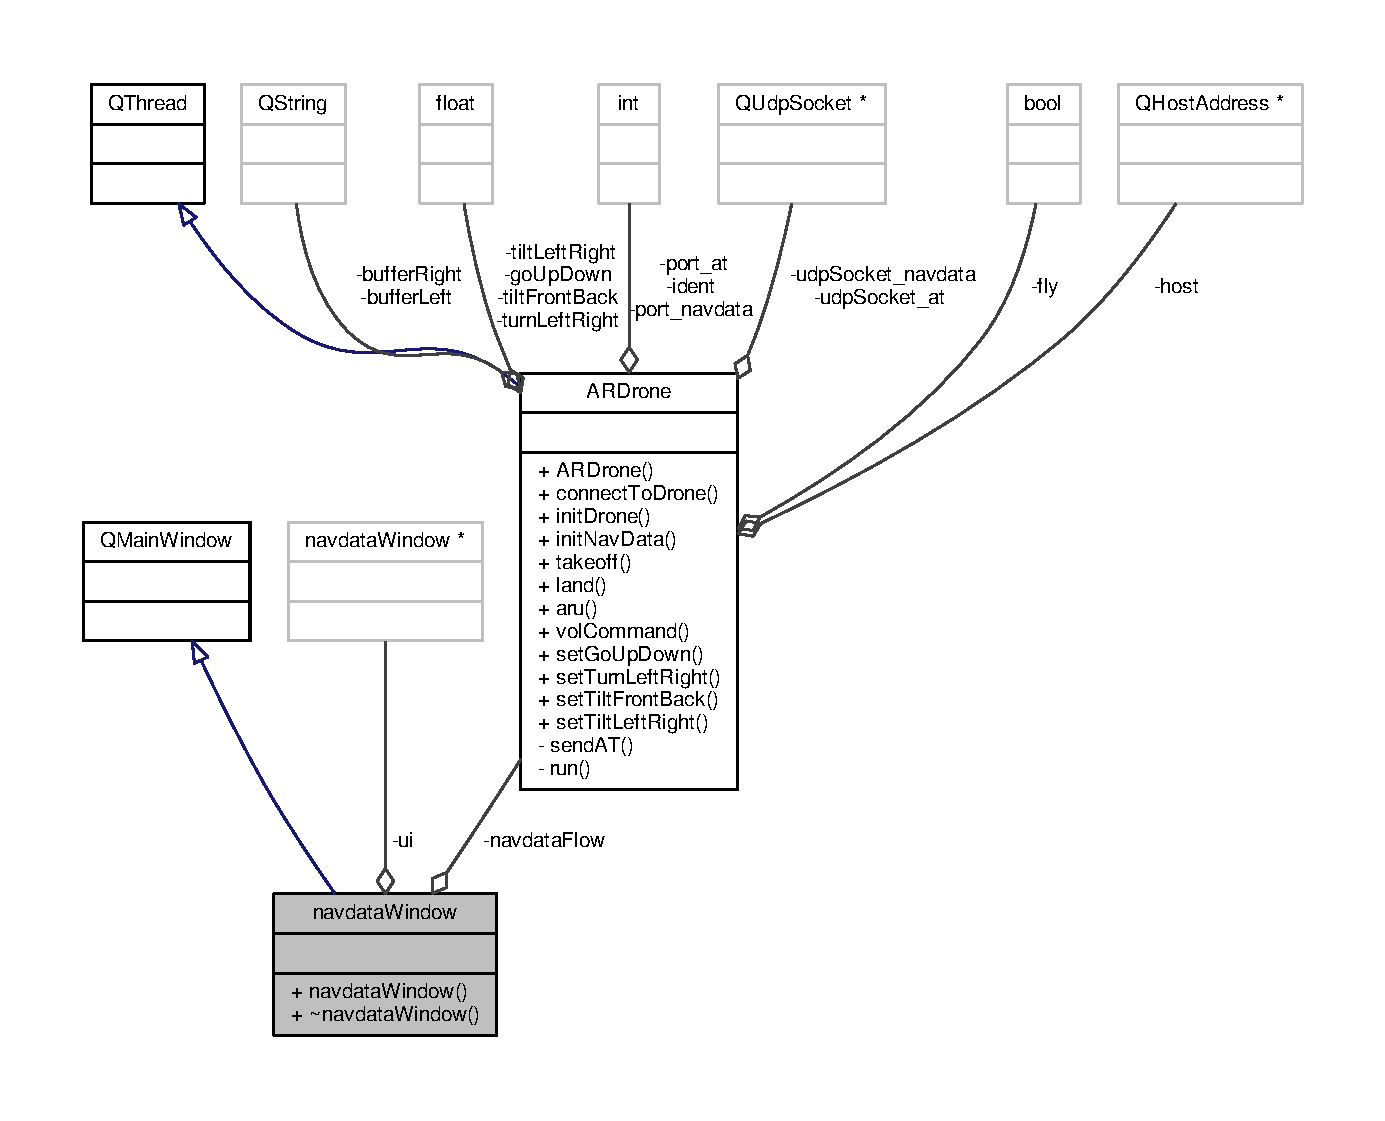
\includegraphics[width=186pt]{classnavdata_window__coll__graph}
\end{center}
\end{figure}
\subsection*{Fonctions membres publiques}
\begin{DoxyCompactItemize}
\item 
\hyperlink{classnavdata_window_a5e017b35b55ad954e54244cc284b1f5a}{navdata\-Window} (Q\-Widget $\ast$parent=0)
\item 
\hyperlink{classnavdata_window_a33a8fdbabc0661a1ee5c18c7de33440e}{$\sim$navdata\-Window} ()
\end{DoxyCompactItemize}


\subsection{Description détaillée}


Définition à la ligne 11 du fichier navdatawindow.\-h.



\subsection{Documentation des constructeurs et destructeur}
\hypertarget{classnavdata_window_a5e017b35b55ad954e54244cc284b1f5a}{\index{navdata\-Window@{navdata\-Window}!navdata\-Window@{navdata\-Window}}
\index{navdata\-Window@{navdata\-Window}!navdataWindow@{navdata\-Window}}
\subsubsection[{navdata\-Window}]{\setlength{\rightskip}{0pt plus 5cm}{\bf navdata\-Window} (
\begin{DoxyParamCaption}
\item[{Q\-Widget $\ast$}]{parent = {\ttfamily 0}}
\end{DoxyParamCaption}
)\hspace{0.3cm}{\ttfamily [explicit]}}}\label{classnavdata_window_a5e017b35b55ad954e54244cc284b1f5a}


Définition à la ligne 4 du fichier navdatawindow.\-cpp.



Voici le graphe d'appel pour cette fonction \-:
\nopagebreak
\begin{figure}[H]
\begin{center}
\leavevmode
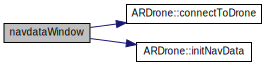
\includegraphics[width=338pt]{classnavdata_window_a5e017b35b55ad954e54244cc284b1f5a_cgraph}
\end{center}
\end{figure}


\hypertarget{classnavdata_window_a33a8fdbabc0661a1ee5c18c7de33440e}{\index{navdata\-Window@{navdata\-Window}!$\sim$navdata\-Window@{$\sim$navdata\-Window}}
\index{$\sim$navdata\-Window@{$\sim$navdata\-Window}!navdataWindow@{navdata\-Window}}
\subsubsection[{$\sim$navdata\-Window}]{\setlength{\rightskip}{0pt plus 5cm}$\sim${\bf navdata\-Window} (
\begin{DoxyParamCaption}
{}
\end{DoxyParamCaption}
)}}\label{classnavdata_window_a33a8fdbabc0661a1ee5c18c7de33440e}


Définition à la ligne 14 du fichier navdatawindow.\-cpp.



La documentation de cette classe a été générée à partir des fichiers suivants \-:\begin{DoxyCompactItemize}
\item 
/media/\-D\-E\-V\-E\-L/\-Projet\-I\-U\-T/\-Drone\-Wifi/sources/keyboard\-Command/\hyperlink{navdatawindow_8h}{navdatawindow.\-h}\item 
/media/\-D\-E\-V\-E\-L/\-Projet\-I\-U\-T/\-Drone\-Wifi/sources/keyboard\-Command/\hyperlink{navdatawindow_8cpp}{navdatawindow.\-cpp}\end{DoxyCompactItemize}

\hypertarget{class_q_main_window}{\section{Référence de la classe Q\-Main\-Window}
\label{class_q_main_window}\index{Q\-Main\-Window@{Q\-Main\-Window}}
}


Graphe d'héritage de Q\-Main\-Window\-:
\nopagebreak
\begin{figure}[H]
\begin{center}
\leavevmode
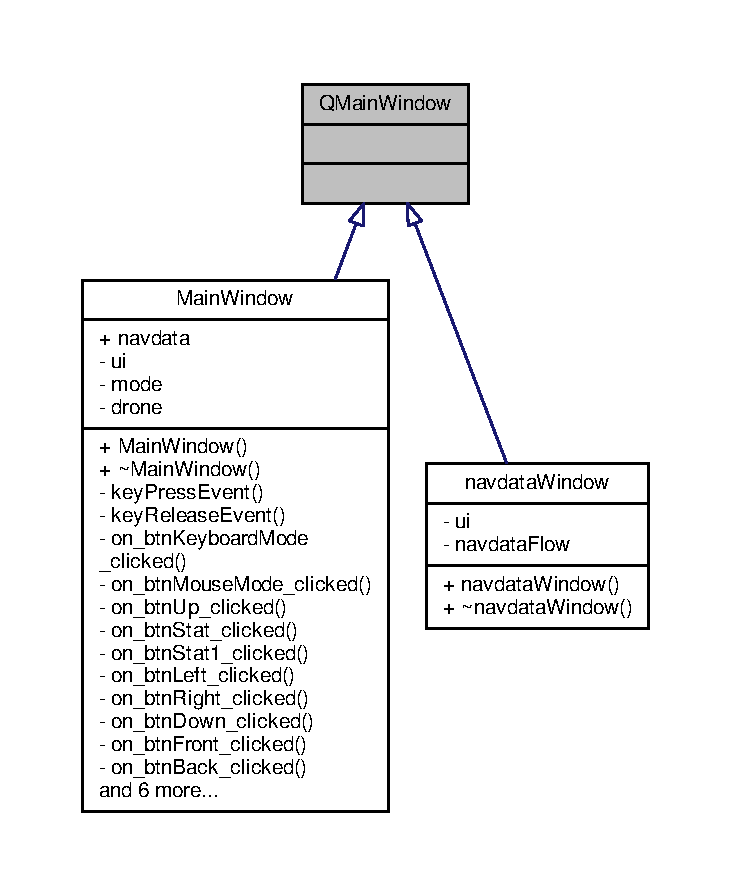
\includegraphics[width=299pt]{class_q_main_window__inherit__graph}
\end{center}
\end{figure}


Graphe de collaboration de Q\-Main\-Window\-:
\nopagebreak
\begin{figure}[H]
\begin{center}
\leavevmode
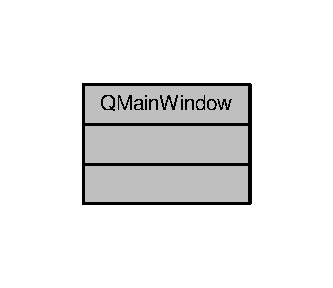
\includegraphics[width=160pt]{class_q_main_window__coll__graph}
\end{center}
\end{figure}


La documentation de cette classe a été générée à partir du fichier suivant \-:\begin{DoxyCompactItemize}
\item 
/media/\-D\-E\-V\-E\-L/\-Projet\-I\-U\-T/\-Drone\-Wifi/sources/keyboard\-Command/\hyperlink{mainwindow_8h}{mainwindow.\-h}\end{DoxyCompactItemize}

\hypertarget{class_q_thread}{\section{Référence de la classe Q\-Thread}
\label{class_q_thread}\index{Q\-Thread@{Q\-Thread}}
}


Graphe d'héritage de Q\-Thread\-:
\nopagebreak
\begin{figure}[H]
\begin{center}
\leavevmode
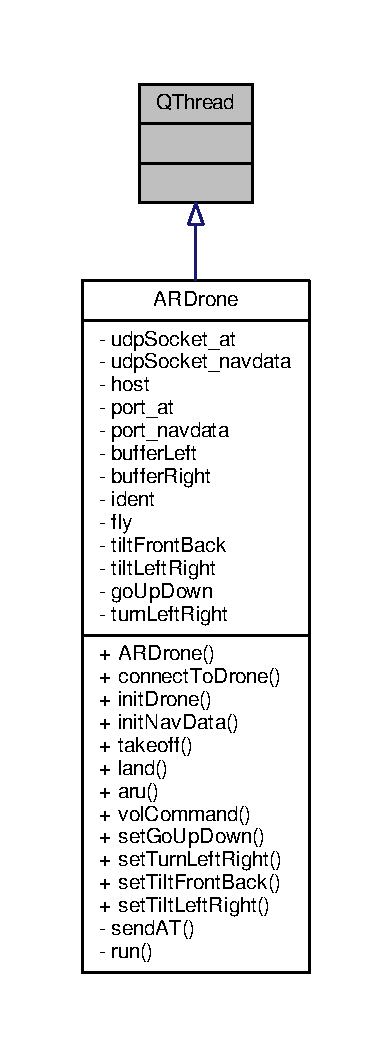
\includegraphics[width=184pt]{class_q_thread__inherit__graph}
\end{center}
\end{figure}


Graphe de collaboration de Q\-Thread\-:
\nopagebreak
\begin{figure}[H]
\begin{center}
\leavevmode
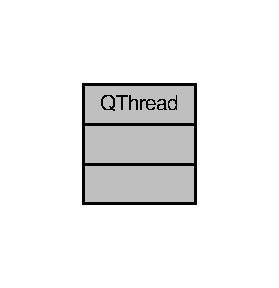
\includegraphics[width=134pt]{class_q_thread__coll__graph}
\end{center}
\end{figure}


La documentation de cette classe a été générée à partir du fichier suivant \-:\begin{DoxyCompactItemize}
\item 
/media/\-D\-E\-V\-E\-L/\-Projet\-I\-U\-T/\-Drone\-Wifi/sources/keyboard\-Command/\hyperlink{ardrone_8h}{ardrone.\-h}\end{DoxyCompactItemize}

\chapter{Documentation des fichiers}
\hypertarget{ardrone_8cpp}{\section{Référence du fichier /media/\-D\-E\-V\-E\-L/\-Projet\-I\-U\-T/\-Drone\-Wifi/sources/keyboard\-Command/ardrone.cpp}
\label{ardrone_8cpp}\index{/media/\-D\-E\-V\-E\-L/\-Projet\-I\-U\-T/\-Drone\-Wifi/sources/keyboard\-Command/ardrone.\-cpp@{/media/\-D\-E\-V\-E\-L/\-Projet\-I\-U\-T/\-Drone\-Wifi/sources/keyboard\-Command/ardrone.\-cpp}}
}
{\ttfamily \#include \char`\"{}ardrone.\-h\char`\"{}}\\*
Graphe des dépendances par inclusion de ardrone.\-cpp\-:
\nopagebreak
\begin{figure}[H]
\begin{center}
\leavevmode
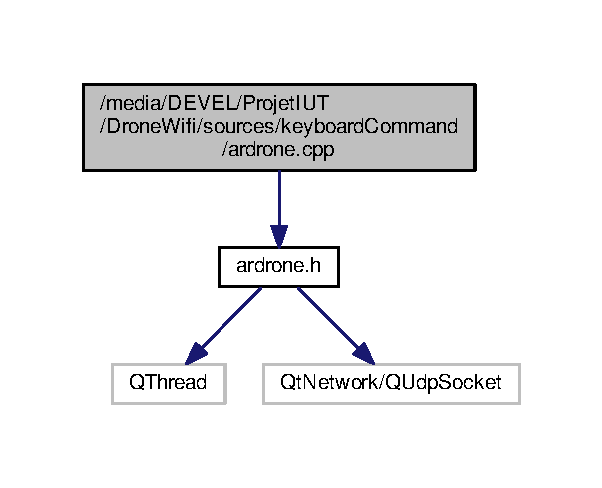
\includegraphics[width=289pt]{ardrone_8cpp__incl}
\end{center}
\end{figure}

\hypertarget{ardrone_8h}{\section{Référence du fichier /media/\-D\-E\-V\-E\-L/\-Projet\-I\-U\-T/\-Drone\-Wifi/sources/keyboard\-Command/ardrone.h}
\label{ardrone_8h}\index{/media/\-D\-E\-V\-E\-L/\-Projet\-I\-U\-T/\-Drone\-Wifi/sources/keyboard\-Command/ardrone.\-h@{/media/\-D\-E\-V\-E\-L/\-Projet\-I\-U\-T/\-Drone\-Wifi/sources/keyboard\-Command/ardrone.\-h}}
}
{\ttfamily \#include $<$Q\-Thread$>$}\\*
{\ttfamily \#include $<$Qt\-Network/\-Q\-Udp\-Socket$>$}\\*
Graphe des dépendances par inclusion de ardrone.\-h\-:
\nopagebreak
\begin{figure}[H]
\begin{center}
\leavevmode
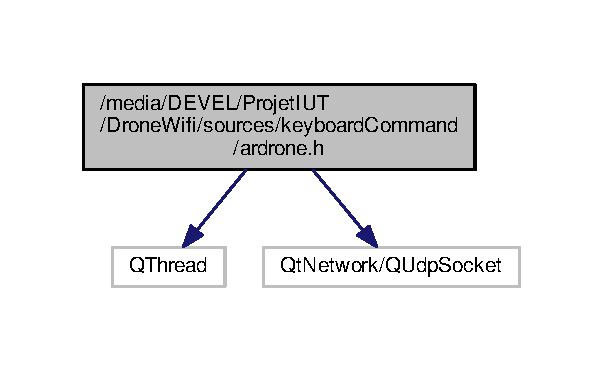
\includegraphics[width=289pt]{ardrone_8h__incl}
\end{center}
\end{figure}
Ce graphe montre quels fichiers incluent directement ou indirectement ce fichier \-:
\nopagebreak
\begin{figure}[H]
\begin{center}
\leavevmode
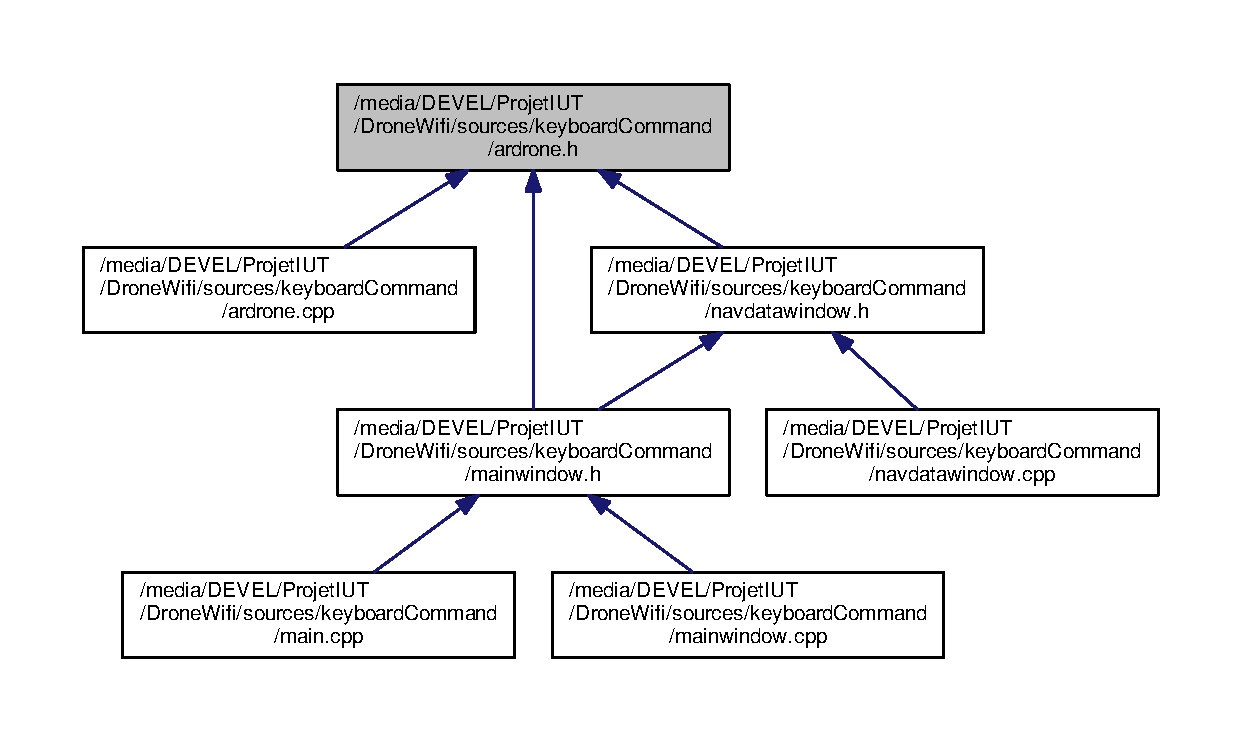
\includegraphics[width=350pt]{ardrone_8h__dep__incl}
\end{center}
\end{figure}
\subsection*{Structures de données}
\begin{DoxyCompactItemize}
\item 
class \hyperlink{class_a_r_drone}{A\-R\-Drone}
\end{DoxyCompactItemize}

\hypertarget{main_8cpp}{\section{Référence du fichier /media/\-D\-E\-V\-E\-L/\-Projet\-I\-U\-T/\-Drone\-Wifi/sources/keyboard\-Command/main.cpp}
\label{main_8cpp}\index{/media/\-D\-E\-V\-E\-L/\-Projet\-I\-U\-T/\-Drone\-Wifi/sources/keyboard\-Command/main.\-cpp@{/media/\-D\-E\-V\-E\-L/\-Projet\-I\-U\-T/\-Drone\-Wifi/sources/keyboard\-Command/main.\-cpp}}
}
{\ttfamily \#include \char`\"{}mainwindow.\-h\char`\"{}}\\*
{\ttfamily \#include $<$Q\-Application$>$}\\*
Graphe des dépendances par inclusion de main.\-cpp\-:
\nopagebreak
\begin{figure}[H]
\begin{center}
\leavevmode
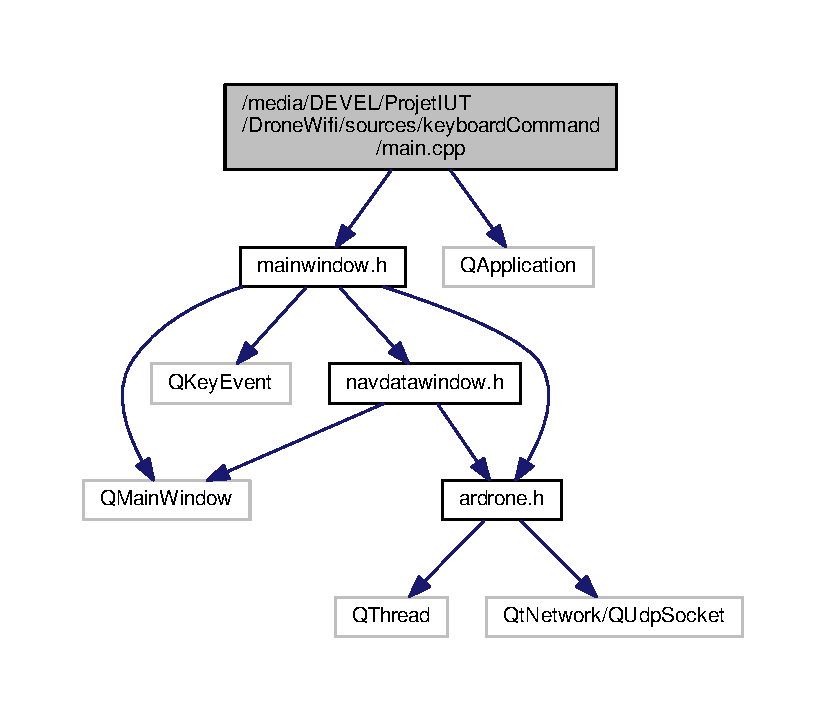
\includegraphics[width=350pt]{main_8cpp__incl}
\end{center}
\end{figure}
\subsection*{Fonctions}
\begin{DoxyCompactItemize}
\item 
int \hyperlink{main_8cpp_a0ddf1224851353fc92bfbff6f499fa97}{main} (int argc, char $\ast$argv\mbox{[}$\,$\mbox{]})
\end{DoxyCompactItemize}


\subsection{Documentation des fonctions}
\hypertarget{main_8cpp_a0ddf1224851353fc92bfbff6f499fa97}{\index{main.\-cpp@{main.\-cpp}!main@{main}}
\index{main@{main}!main.cpp@{main.\-cpp}}
\subsubsection[{main}]{\setlength{\rightskip}{0pt plus 5cm}int main (
\begin{DoxyParamCaption}
\item[{int}]{argc, }
\item[{char $\ast$}]{argv\mbox{[}$\,$\mbox{]}}
\end{DoxyParamCaption}
)}}\label{main_8cpp_a0ddf1224851353fc92bfbff6f499fa97}


Définition à la ligne 4 du fichier main.\-cpp.


\hypertarget{mainwindow_8cpp}{\section{Référence du fichier /media/\-D\-E\-V\-E\-L/\-Projet\-I\-U\-T/\-Drone\-Wifi/sources/keyboard\-Command/mainwindow.cpp}
\label{mainwindow_8cpp}\index{/media/\-D\-E\-V\-E\-L/\-Projet\-I\-U\-T/\-Drone\-Wifi/sources/keyboard\-Command/mainwindow.\-cpp@{/media/\-D\-E\-V\-E\-L/\-Projet\-I\-U\-T/\-Drone\-Wifi/sources/keyboard\-Command/mainwindow.\-cpp}}
}
{\ttfamily \#include \char`\"{}mainwindow.\-h\char`\"{}}\\*
{\ttfamily \#include \char`\"{}ui\-\_\-mainwindow.\-h\char`\"{}}\\*
Graphe des dépendances par inclusion de mainwindow.\-cpp\-:
\nopagebreak
\begin{figure}[H]
\begin{center}
\leavevmode
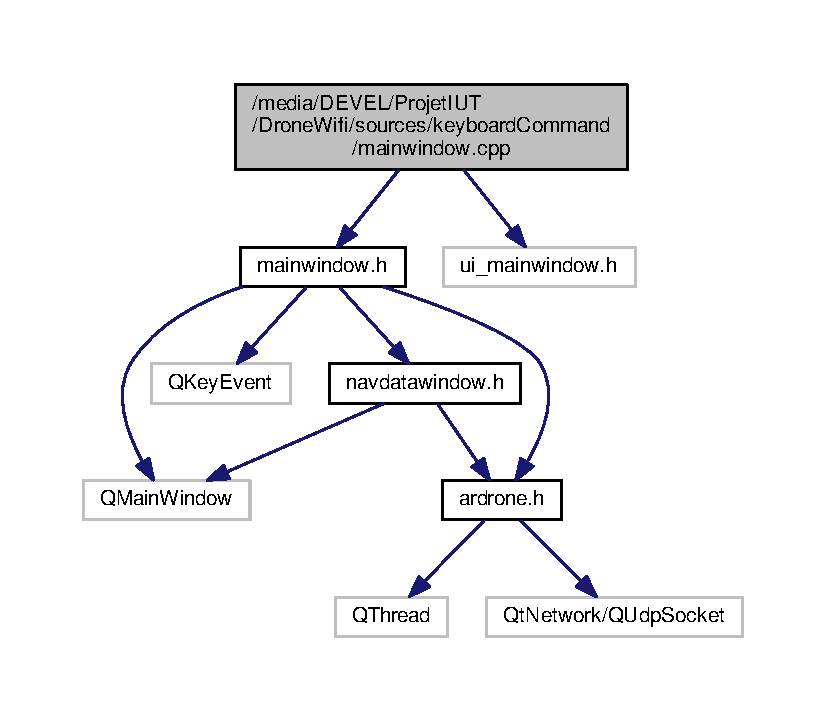
\includegraphics[width=350pt]{mainwindow_8cpp__incl}
\end{center}
\end{figure}

\hypertarget{mainwindow_8h}{\section{Référence du fichier /media/\-D\-E\-V\-E\-L/\-Projet\-I\-U\-T/\-Drone\-Wifi/sources/keyboard\-Command/mainwindow.h}
\label{mainwindow_8h}\index{/media/\-D\-E\-V\-E\-L/\-Projet\-I\-U\-T/\-Drone\-Wifi/sources/keyboard\-Command/mainwindow.\-h@{/media/\-D\-E\-V\-E\-L/\-Projet\-I\-U\-T/\-Drone\-Wifi/sources/keyboard\-Command/mainwindow.\-h}}
}
{\ttfamily \#include $<$Q\-Main\-Window$>$}\\*
{\ttfamily \#include $<$Q\-Key\-Event$>$}\\*
{\ttfamily \#include \char`\"{}ardrone.\-h\char`\"{}}\\*
{\ttfamily \#include \char`\"{}navdatawindow.\-h\char`\"{}}\\*
Graphe des dépendances par inclusion de mainwindow.\-h\-:
\nopagebreak
\begin{figure}[H]
\begin{center}
\leavevmode
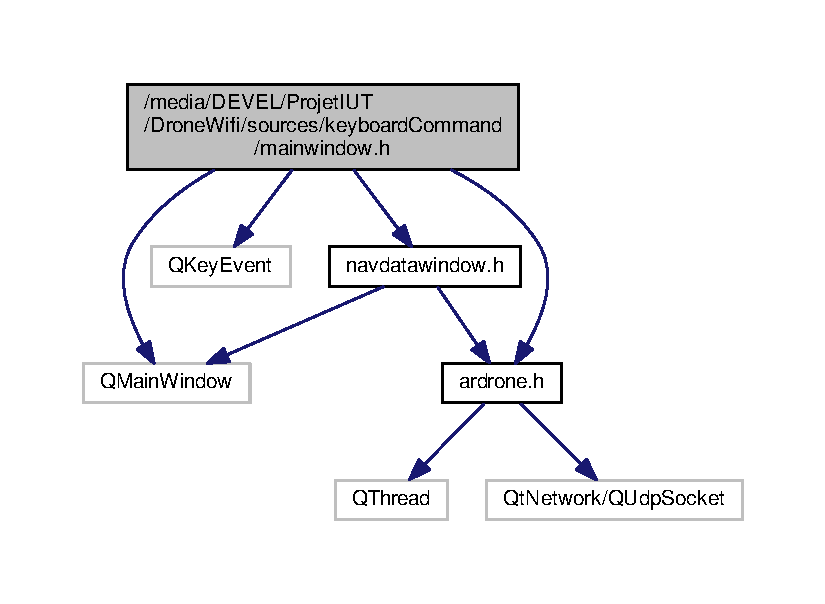
\includegraphics[width=350pt]{mainwindow_8h__incl}
\end{center}
\end{figure}
Ce graphe montre quels fichiers incluent directement ou indirectement ce fichier \-:
\nopagebreak
\begin{figure}[H]
\begin{center}
\leavevmode
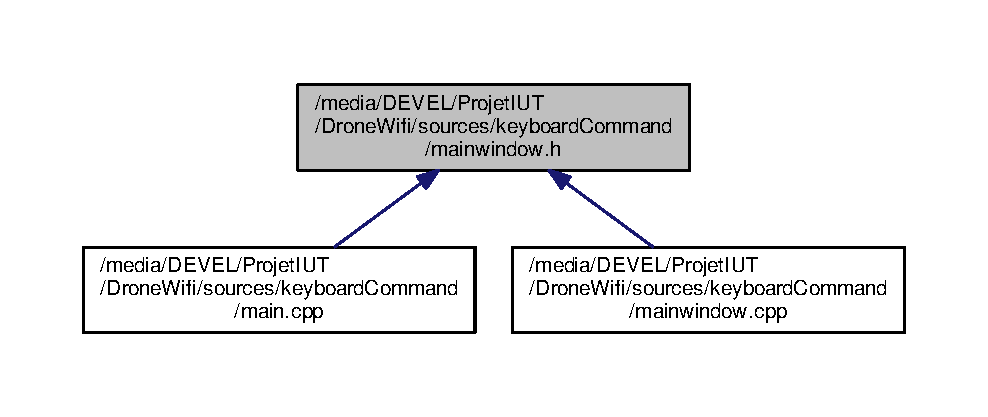
\includegraphics[width=350pt]{mainwindow_8h__dep__incl}
\end{center}
\end{figure}
\subsection*{Classes}
\begin{DoxyCompactItemize}
\item 
class \hyperlink{class_main_window}{Main\-Window}
\end{DoxyCompactItemize}
\subsection*{Espaces de nommage}
\begin{DoxyCompactItemize}
\item 
namespace \hyperlink{namespace_ui}{Ui}
\end{DoxyCompactItemize}

\hypertarget{navdatawindow_8cpp}{\section{Référence du fichier /media/\-D\-E\-V\-E\-L/\-Projet\-I\-U\-T/\-Drone\-Wifi/sources/keyboard\-Command/navdatawindow.cpp}
\label{navdatawindow_8cpp}\index{/media/\-D\-E\-V\-E\-L/\-Projet\-I\-U\-T/\-Drone\-Wifi/sources/keyboard\-Command/navdatawindow.\-cpp@{/media/\-D\-E\-V\-E\-L/\-Projet\-I\-U\-T/\-Drone\-Wifi/sources/keyboard\-Command/navdatawindow.\-cpp}}
}
{\ttfamily \#include \char`\"{}navdatawindow.\-h\char`\"{}}\\*
{\ttfamily \#include \char`\"{}ui\-\_\-navdatawindow.\-h\char`\"{}}\\*
Graphe des dépendances par inclusion de navdatawindow.\-cpp\-:
\nopagebreak
\begin{figure}[H]
\begin{center}
\leavevmode
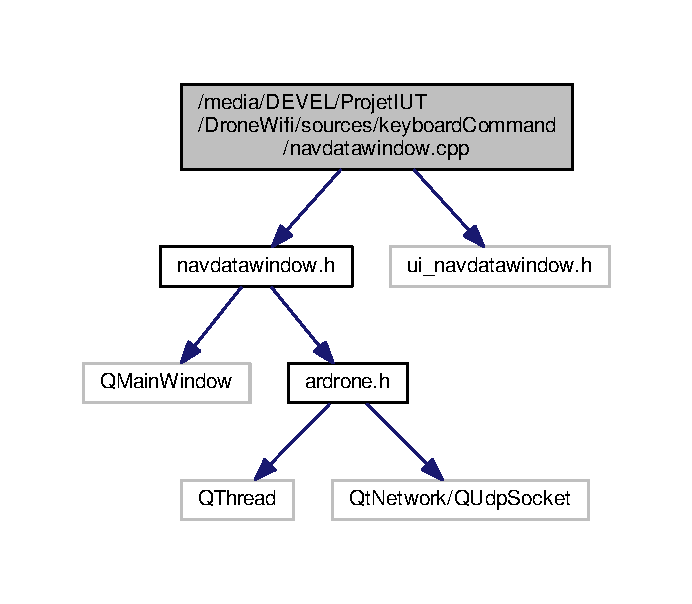
\includegraphics[width=332pt]{navdatawindow_8cpp__incl}
\end{center}
\end{figure}

\hypertarget{navdatawindow_8h}{\section{Référence du fichier /media/\-D\-E\-V\-E\-L/\-Projet\-I\-U\-T/\-Drone\-Wifi/sources/keyboard\-Command/navdatawindow.h}
\label{navdatawindow_8h}\index{/media/\-D\-E\-V\-E\-L/\-Projet\-I\-U\-T/\-Drone\-Wifi/sources/keyboard\-Command/navdatawindow.\-h@{/media/\-D\-E\-V\-E\-L/\-Projet\-I\-U\-T/\-Drone\-Wifi/sources/keyboard\-Command/navdatawindow.\-h}}
}
{\ttfamily \#include $<$Q\-Main\-Window$>$}\\*
{\ttfamily \#include \char`\"{}ardrone.\-h\char`\"{}}\\*
Graphe des dépendances par inclusion de navdatawindow.\-h\-:
\nopagebreak
\begin{figure}[H]
\begin{center}
\leavevmode
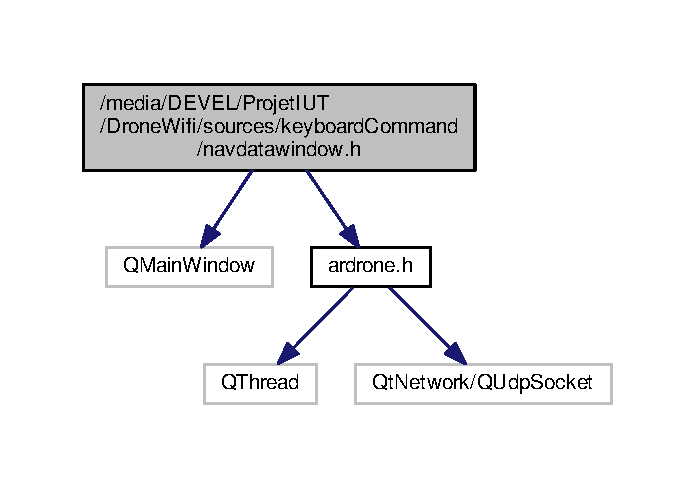
\includegraphics[width=333pt]{navdatawindow_8h__incl}
\end{center}
\end{figure}
Ce graphe montre quels fichiers incluent directement ou indirectement ce fichier \-:
\nopagebreak
\begin{figure}[H]
\begin{center}
\leavevmode
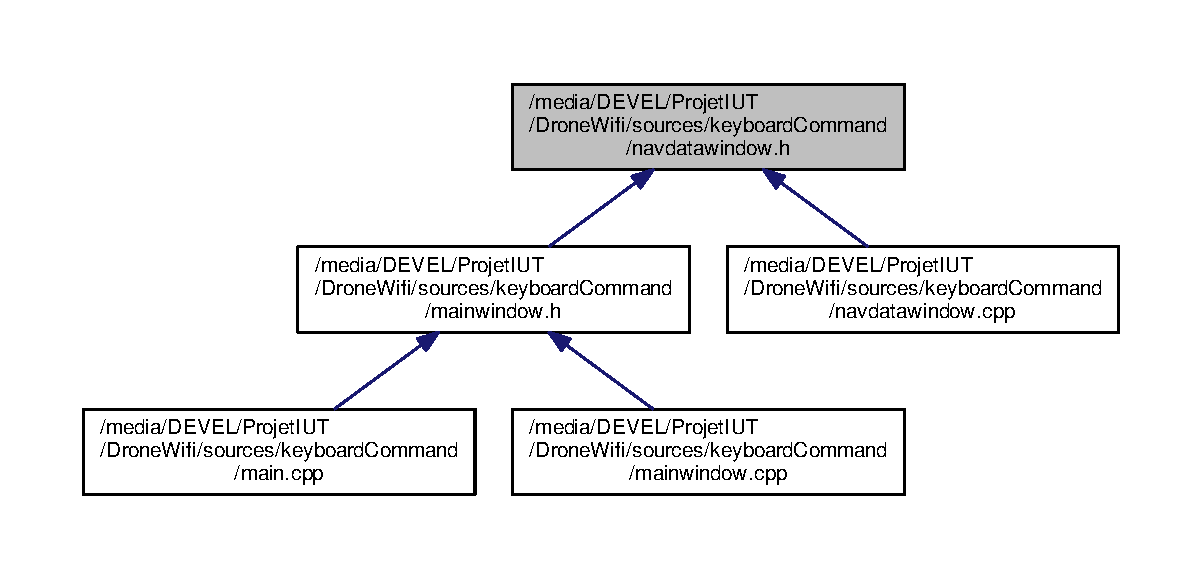
\includegraphics[width=350pt]{navdatawindow_8h__dep__incl}
\end{center}
\end{figure}
\subsection*{Classes}
\begin{DoxyCompactItemize}
\item 
class \hyperlink{classnavdata_window}{navdata\-Window}
\end{DoxyCompactItemize}
\subsection*{Espaces de nommage}
\begin{DoxyCompactItemize}
\item 
namespace \hyperlink{namespace_ui}{Ui}
\end{DoxyCompactItemize}

\addcontentsline{toc}{part}{Index}
\printindex
\end{document}
